%%%%%%%%%%%%%%%%%%%%%%%%%%%%%%%%%%%%%%%%%%%%%%%%%%%%%%%%%%%%%%%%%%%%%%%%%%%%%%%
%%                                                                   CERN & LHC
%%%%%%%%%%%%%%%%%%%%%%%%%%%%%%%%%%%%%%%%%%%%%%%%%%%%%%%%%%%%%%%%%%%%%%%%%%%%%%%
%%                                             Few words about CERN and the LHC

\chapter{Experimenteller Aufbau}
\label{experimenteller_aufbau}

\begin{quote}
    In diesem Kapitel sollen die Grundzüge des Experimentes dargelegt werden.
    Aufgrund der überaus hohen Komplexität wird an vielen Stellen lediglich die
    Idee oder das Prinzip erläutert, da eine detailiertere Betrachtung den
    Rahmen dieser Arbeit übersteigen würde. Im ersten Abschnitt wird kurz der
    Teilchenbeschleuniger \acs{LHC} vorgestellt, woran sich die Beschreibung
    des Aufbaus und der Funktionsweise des ATLAS-Detektors anschließt. Da die
    Grundlage dieser Arbeit der Nachweis von Elektronen und Positronen ist,
    wird gegen Ende des Kapitel noch die Art und Weise beschrieben, wie diese
    in ATLAS identifiziert und rekonstruiert werden.
\end{quote}



%______________________________________________________________________________
%                                                                    CERN & LHC
%
\section{Der Large Hadron Collider}
\label{lhc}

Der \acf{LHC} ist der derzeit leistungsstärkste Teilchenbeschleuniger der Welt
und steht am CERN\footnote{\acf{CERN}} nahe Genf in der Schweiz. Die
Fertigstellung erfolgte 2008 unter Beiteiligung von über einhundert Nationen.
Der \ac{LHC} ist ein Hadronen-Speicherring mit knapp $27\;\kilo\meter$ Umfang,
der in den Tunnel des Vorgänger-Beschleunigers LEP\footnote{\acf{LEP}} zwischen
50m und 100m unter der Erdoberfläche, gebaut wurde. Im Kern ist der
\ac{LHC} ein Synchrotron, dass Protonen oder Blei-Ionen in gegenläufigen
Teilchenstrahlen auf annähernd Lichtgeschwindigkeit beschleunigt und an
fest definierten Punkten zur Kollision bringt. Zuvor durchlaufen die Teilchen
einige Vorbeschleunigerstufen, die die Teilchen bereits auf eine Energie von
$900\GeV$ bringen, bovir sie in den \ac{LHC} einspeist werden. Die
Kollisionspunkte der Teilchenstrahlen liegen innerhalb der Detektoren der
Experimente. Die vier größten Experimente sind \acs{ATLAS}, CMS, ALICE und
LHCb, deren Lage am Beschnleunigerring in Abbildung \ref{fig:LHC} zu sehen ist.

\begin{figure}[h]
    \centering
    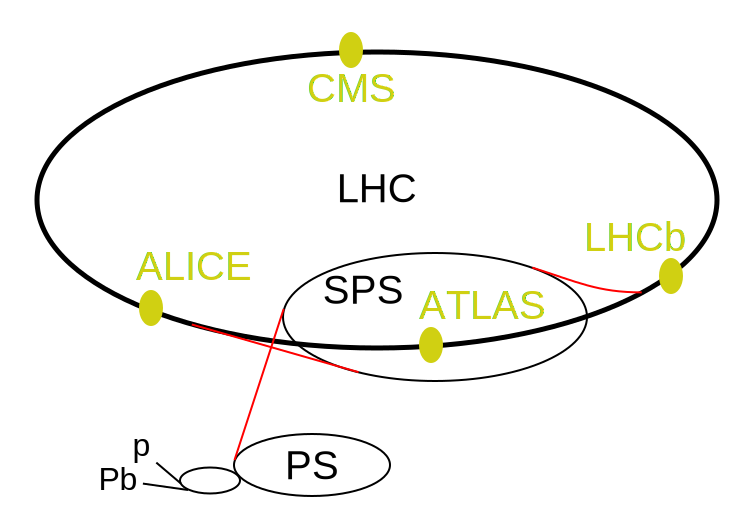
\includegraphics[width=0.5\textwidth]{img/LHC}
    \caption[Zeichnung des LHC mit Vorbeschleunigern und Experimenten]
        {Schematische Zeichnung des LHC mit den vier größten Experimenten und
        den letzten Vorbeschleunigerstufen (PS, SPS)}
    \label{fig:LHC}
\end{figure}

Der \ac{LHC} wird prinzipiell in zwei Modi betrieben: Proton-Proton Kollisionen
oder Proton-Blei Kollisionen. Aufgrund der Relevanz für die vorliegende Arbeit
wird im Folgenden auschließlich auf erstgenannten Modus eingegangen. In
Proton-Proton Kollisionen erreichte der \ac{LHC} zuletzt Schwerpunktsenergien
von $8\TeV$ und befindet sich zum Zeitpunkt dieser Arbeit in der ersten großen
Wartungsphase nach deren Abschluss die Design-Schwerpunktsenergie von $14\TeV$
erreicht werden soll.

Die Protonen werden in Paketen, sog. \textit{Bunches} (vom engl. \textit{bunch}
- Bündel) von je etwa $10^{11}$ Teilchen in den \ac{LHC} eingespeist, welche
mit einer Rate von $20\mega\hertz$ in den Teilchendetektoren kollidieren.
Zuvor werden die Pakete durch Magnete auf die Kollisionspunkte fokusiert, um
deren Querschnittsfläche zu minimieren und somit die Luminosität zu maximieren
(siehe Gleichung \ref{eq:collider_lumi}). So konnten bisher Luminositäten von
bis zu $8\cdot 10^{-33} \centi\meter^{-2}\second^{-1}$ erreicht werden.



%______________________________________________________________________________
%                                                            Der ATLAS Detektor
%
\section{Der ATLAS Detektor}
\label{atlas_detector}

% + Skimms und Slimms, D3PD (auch Verweis auf DAQ)
% + GRL, Fills/Runs, LumiBlocks

Der ATLAS Detektor\footnote{\acf{ATLAS}} ist ein Vielzweck Teilchendetektor und
eines der vier Hauptexperimente am \ac{LHC}. Mit $44\meter$ Länge, $25\meter$
Durchmesser und etwa $7000\ton$ Gewicht ist es zugleich auch das größte der
Experimente. Der grundlegende Aufbau gleicht einem Schalenmodell und ist
symmetrisch um die Strahlachse angelegt (siehe Abbildung \ref{fig:atlas}).

\begin{figure}
    \centering
    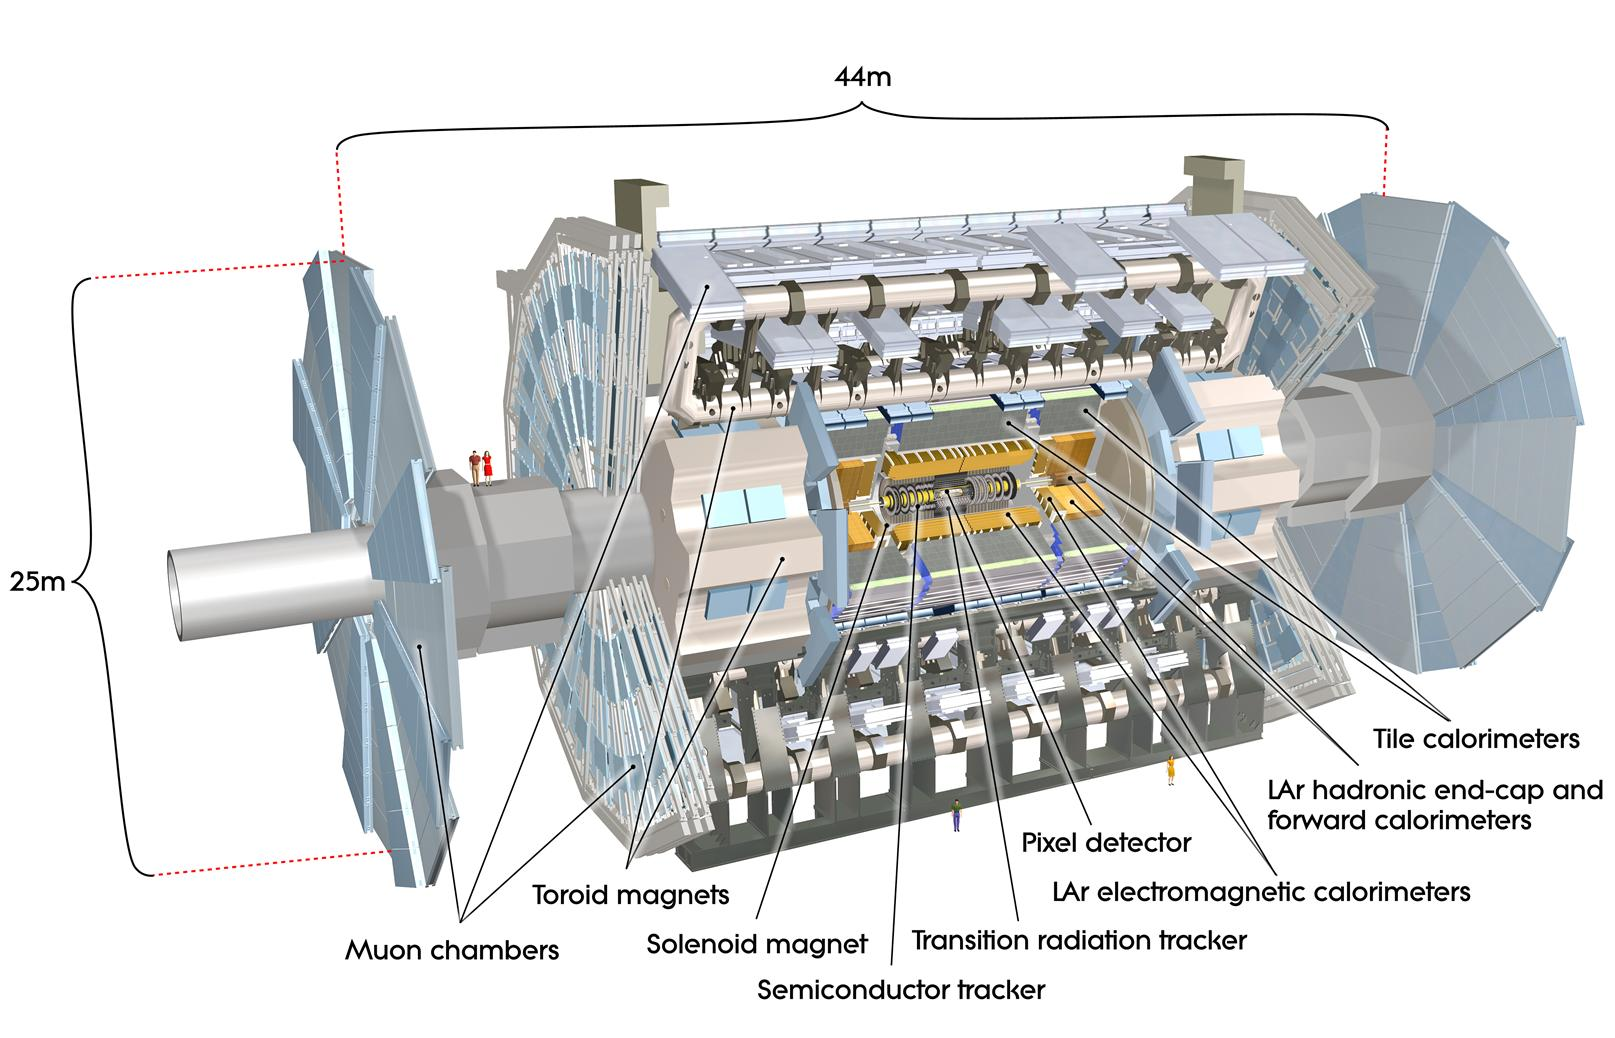
\includegraphics[width=1.0\textwidth]{img/atlas}
    \caption[Aufgeschnittene Darstellung des ATLAS Detektors]
        {Aufgeschnittene Darstellung des ATLAS Detektors}
    \label{fig:atlas}
\end{figure}

Dabei befindet sich unmittelbar um die Strahlachse der innere Detektor zur
Bestimmung der Vertexposition und zur Spurmessung. In diesem Bereich herrscht
ein solenoides Magentfeld von etwa $2\tesla$ Stärke. Den inneren Detektor
umgebend schließen sich das elektromagnetische und das hadronische Kalorimeter
zur Messung der Energie an. Die äußerste Schale stellt das Myon-System dar,
welches von einem toroidalen Magentfeld durchzogen wird.

Bevor die einzelnen Komponenten näher erläutert werden ist es zweckmäßig das in
ATLAS verwendet Koordinatensystem zu definieren. Ausgangspunkt hierfür ist der
nominelle Wechselwirkungspunkt im Zentrum des Detektors, welcher den Nullpunkt
darstellt. Die Strahlachse und zugleich radiale Symmetrieachse des Detektors
wird als z-Achse festgelegt. Die x-Achse zeigt orthogonal zur Strahlachse auf
die Mitte des Beschleuniger-Rings, während die y-Achse noch oben zeigt und
somit ein Rechtssystem entsteht. Aufgrund der symmetrischen Geometrie des
Detektors definiert man nun für Richtungsangaben einen Azimuthwinkel
$\phi$ in der x-y-Ebene um die Strahlachse, wobei die positive x-Achse der
Ebene mit $\phi=0$ entspricht, und die Pseudorapidität $\eta$ anstelle des
Polarwinkels $\theta$:
\begin{equation}
    \eta \; = \; - \ln \left( \tan\frac{\theta}{2} \right)
    \label{eq:eta}
\end{equation}
Die Verwendung der Pseudorapidität ist gebräuchlich, da die Rate der in
Proton-Proton Kollisionen erzeugten Teilchen als Funktion von $\eta$ annähernd
konstant ist. Abstände in der $\eta$-$\phi$ Ebene werden mit
$R=\sqrt{\eta^2-\phi^2}$ angegeben. Wie aus der Definition (\ref{eq:eta})
ersichtlich ist, entspricht $\eta=0$ der Richtung senkrecht zur Strachachse,
während $|\eta| \rightarrow \infty$ mit der Richtung parallel zu selbiger
übereinstimmt.

Im Folgenden werden nun die zum Nachweis von Elektronen relevanten Komponenten
des Detektors und deren Funktionsweise näher erläutert.



\subsection{Innerer Detektor}
\label{inner_detector}

Der innere Detektor bildet das Spurerkennungssystem von ATLAS und besteht im
wesentlichen aus drei Hauptkomponenten. Von innen nach außen folgen der
Pixeldetektor, der Silizium-Streifen Detektor (\acs{SCT})\footnote{\acf{SCT}}
und der Übergangsstrahlungsdetektor (\acs{TRT})\footnote{\acf{TRT}}. Abbildung
\ref{fig:inner_detector} zeigt den Aufbau des inneren Detektors. Seine Aufgabe
ist die Rekonstruktion der Spuren geladener Teilchen, woraus die Position des
Wechselwirkungs-Vertex bestimmt wird. Desweiteren wird aus der durch das
anliegende solenoide Magnetfeld induzierten Krümmung der Teilchenspuren deren
Impuls bestimmt. Ebenso lässt sich auch die Ladung eines Teilchens aus dem
Vorzeichen dieser Krümmung bestimmen.

\begin{figure}
    \centering
    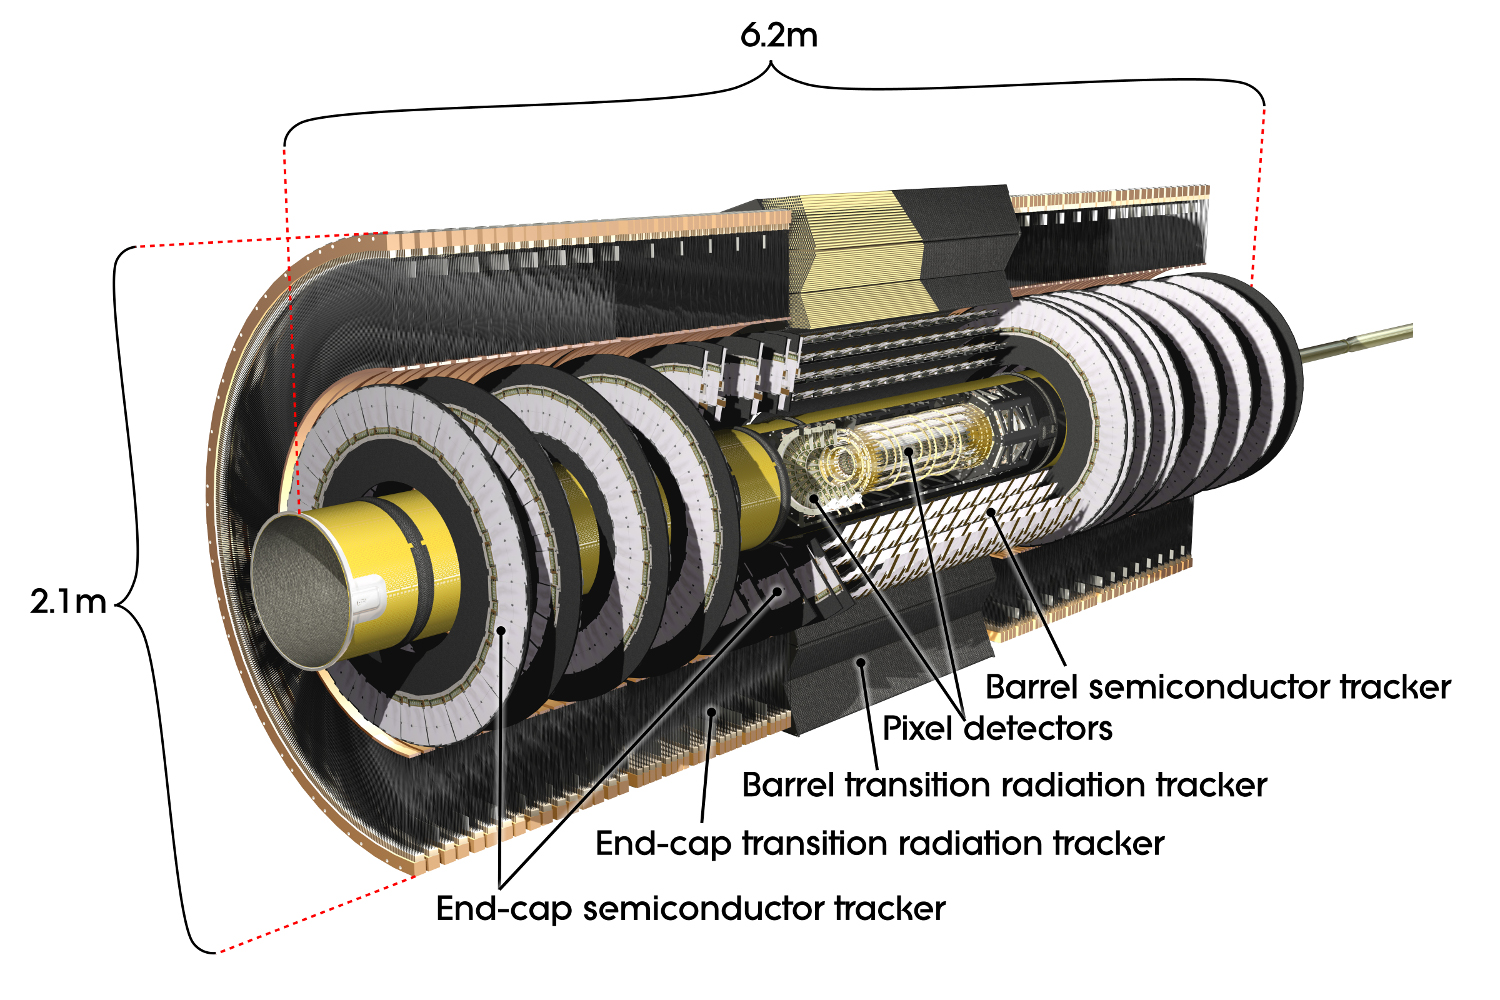
\includegraphics[width=.8\textwidth]{img/inner_detector}
    \caption[Darstellung des inneren Detektors]
        {Aufgeschnittene Darstellung des inneren Detektors}
    \label{fig:inner_detector}
\end{figure}

Der Pixeldetektor besteht aus drei zylindrisch angelegten Lagen von
Silzium-Pixeln im Zentrum, sowie je drei weiteren scheibenförmigen Lagen
konzentrisch angedordnet links und rechts davon. Insgesamt wird so ein Bereich
von $|\eta| < 2.5$ abgedeckt. Die erste zylindrische Lage hat dabei einen
Abstand von gerademal $45\milli\meter$ zur Strahlachse. Die Aufgabe des
Pixeldetektors ist räumliche Auflösung der Teilchenspuren zur Bestimmung des
Primärvertex, also der Position der ursprünglichen Wechselwirkung. Zudem lassen
sich Sekundärvertizes nahe an der Strahlachse erkennen. Diese entstehen, wenn
Teilchen sich als Zwischenprodukte vom Primärvertex entfernen und erst abseits
dessen weiterzerfallen. Da ein solches Verhalten typisch für b-Quarks ist, wird
die erste der drei Pixel-Lagen auch \textit{b-layer} (vom engl. \textit{layer},
Lage) genannt. Der Pixeldetektor erlaubt eine räumliche Auflösung von
$10\micro\meter$ in der $R$-$\phi$ Ebene und $115\micro\meter$ in z-Richtung.

Die nächste Schale bildet der \acf{SCT}, der mit einer Abdeckung von ebenfalls
$|\eta| < 2.5$ aus vier zylindrischen Lagen im Zentrum und neun Lagen auf jeder
Seite in Scheibenform. Auch hier kommen Halbleiter-Detektoren zum Einsatz, die
hier allerdings in Streifenform konstruiert wurden. Da mit größerem Radius die
Dichte der nachzuweisenden Spuren abnimmt ist hier eine Auflösung von
$17\micro\meter \times 580\micro\meter$ in ($R-\phi$) bzw. z-Richtung
ausreichend.

Die letzte Schicht, welche den inneren Detektor abschließt bildet der
\acf{TRT}.  Dieser besteht aus gasgefüllten Driftröhren von je etwa
$4\milli\meter$ Durchmesser, die im Zentrum parallel, an Seiten senkrecht zur
Strahlachse ausgerichtet sind. Der \ac{TRT} deckt dabei einen Bereich von
$\eta<2.0$ ab und erreicht eine Auflösung von $130\micro\meter$ in der
($R-\phi$) Ebene im Zentrum bzw. der ($z-\phi$) Ebene an den Seiten. Passiert
ein geladenes Teilchen die Driftröhren ionisiert es deren Gas. Eine
Hochspannungs-Elektrode in der Mitte jeder Röhre saugt die Ionen ab und erzeugt
so einen messbaren Strom. Die Driftröhren sind umgeben von einem Medium, dass
proportional zum Lorentz-Faktor $\gamma=E/m$ des passierenden Teilchens
zusätzlich Übergangsstrahlung erzeugt wodurch der Ionistionsprozess verstärkt
wird. Elektronen erzeugen deshalb aufgrund ihrer geringeren Masse deutlich mehr
Übergangsstrahlung als dies beispielsweise geladene Hadronen tun.



\subsection{Kalorimeter}
\label{calorimeter}

Den inneren Detektor umgebend, folgt zunächst das elektromagnetische
Kalorimeter zur Messung der Energie von Elektronen und Photonen und
anschließend das hadronische Kalorimeter, das die selbe Aufgabe für Mesonen und
Baryonen Teilchen übernimmt (siehe Abbildung \ref{fig:calorimeter}).

\begin{figure}
    \centering
    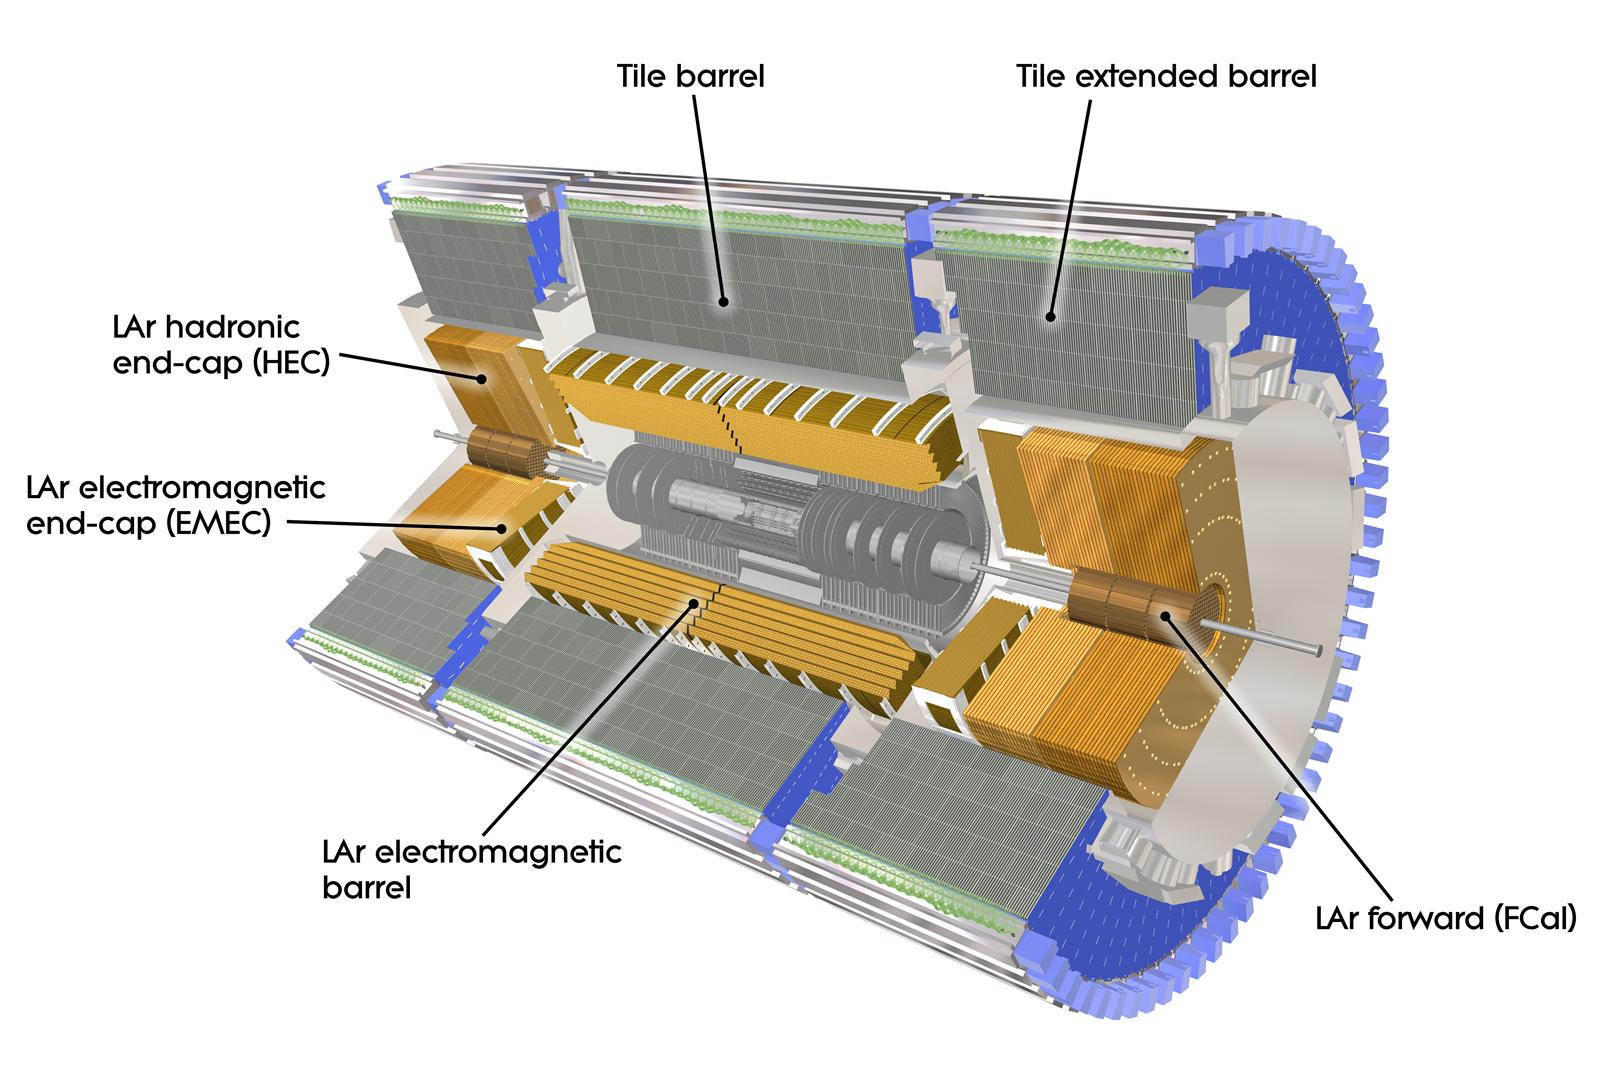
\includegraphics[width=0.8\textwidth]{img/calorimeter}
    \caption[Darstellung der Kalorimeter]
        {Aufgeschnittene Darstellung des elektromagnetischen und hadronischen
        Kalorimeters}
    \label{fig:calorimeter}
\end{figure}

Die Geometrie der Kalorimeter macht die Definition einiger Begriffe sinnvoll,
welche die Bezeichnung der einzelnen Bereiche der Kalorimeter vereinfacht. So
spricht man im Bereich von $|\eta|<2.5$ von sogenannten \emph{Zentral-Bereich},
während die Regionen mit $|\eta| > 2.5$ als \emph{Vorwärts-Bereich}
bezeichnet\footnote{Der Verwendung des Betrages von $\eta$ impliziert
tatsächlich zwei Bereiche, die \textit{vorwärts} genannt werden. Da allerdings
die Seite des Detektors i.d.R irrelevant ist, wird im Folgenden nur von 
\textit{dem Vorwärts-Bereich} im Sinne beider Seiten gesprochen. Andernfalls
erfolgt ein expliziter Hinweis auf die Unterscheidung der beiden Regionen.}
werden.

\subsubsection{Das elektromagnetische Kalorimeter}
Das elektromagnetische Kalorimeter besteht in seiner inneren Struktur aus sich
abwechselnden Schichten von Absorbermaterial und aktivem Nachweismedium. Für
letztgenanntes wird flüssiges Argon verwendet, während als Absorbermaterial in
den meisten Bereichen des Kalorimeters Blei und nur im äußersten
Vorwärts-Bereich Kupfer bzw. Wolfram gewählt wird.

Trifft ein Elektron auf das Kalorimeter, emittiert es in den Absorberschichten
energiereiche Photonen durch Bremsstrahlung. Diese erzeugen durch Paarbildung
weitere Elektronen und Positronen, die ihrerseits wiederum Photonen abstrahlen.
Der Prozess wiederholt sich dabei solange, bis die Energie der
Bremsstrahlungsphotonen zu gering ist, um neue Elektron-Positron Paarbildungen
anzustoßen\footnote{die für den Paarbildungsprozess nötige Energie beträgt
mindestens die doppelte Elektron-Ruhemasse}. Aufgrund dieser fortlaufenden
Verzweigung nennt man die Gesamtheit der erzeugten Sekundärteilchen auch
Teilchenschauer. Während des gesamten Prozess ionisieren die geladenen Teilchen
des Schauers das flüssige Argon, während ein durch Hochspannung erzeugtes
elektrisches Feld sorgt dafür, dass die erzeugten Ladungsträger zu den
Elektroden driften, wo sie einen messbaren elektrischen Strom proportional zur
Energie des ionisierenden Teilchen induzieren.

Zusätzlich zur deponierten Energie des eintreffenden Elektrons wird vom
Kalorimeter auch die Ortsinformation des Teilchenschauers aufgelöst. Zu diesem
Zweck ist das Kalorimeter in einzelne Zellen aufgeteilt, die getrennt
voneinander lediglich ihren Teil der im Schauer deponierten Energie bestimmen.
So kann nicht nur die Position, sondern auch die Form des Schauers analysiert
werden. Die räumliche Ausdehnung eines Teilchenschauers wird für gewöhnlich in
Strahlungslängen $X_0$ des Elektrons angegeben, also der Entfernung, nach der
die Energie eines Elektrons durch Bremsstrahlungsprozesse auf $1/e$ seiner
ursprünglichen Energie abgefallen ist. Ebenso werden die Abmessungen des
Kalorimeters selbst zumeist in der gleichen Einheit spezifiziert.

Das elektromagnetische Kalorimeter kann in drei Bereiche unterteilt werden, das
sogenannte \textit{Barrel} (vom engl. \textit{barrel}, Fass), die Endkappen
und die Vorwärts-Kalorimeter. Das Barrel besteht aus zwei baugleichen
zylinderförmigen Teilen, die konzentrisch um die Strahlachse und den inneren
Detektor angelegt sind und bei $\eta=0$ stirnseitig mit wenigen Millimetern
Abstand zusammenliegen (siehe Abbildung \ref{fig:calorimeter}). Das Barrel
überdeckt dabei einen Bereich von $|\eta| < 1.475$. Die Bleiabsorberschichten
sind in der Form eines Akkordeons übereinander gestapelt und parallel zur
Strahlachse ausgerichtet, wie in Abbildung \ref{fig:accordion} zu sehen ist.
Auf diese Weise wird eine vollständige Abdeckung im Azimuthwinkel $\phi$
erreicht.

\begin{figure}[h]
    \centering
    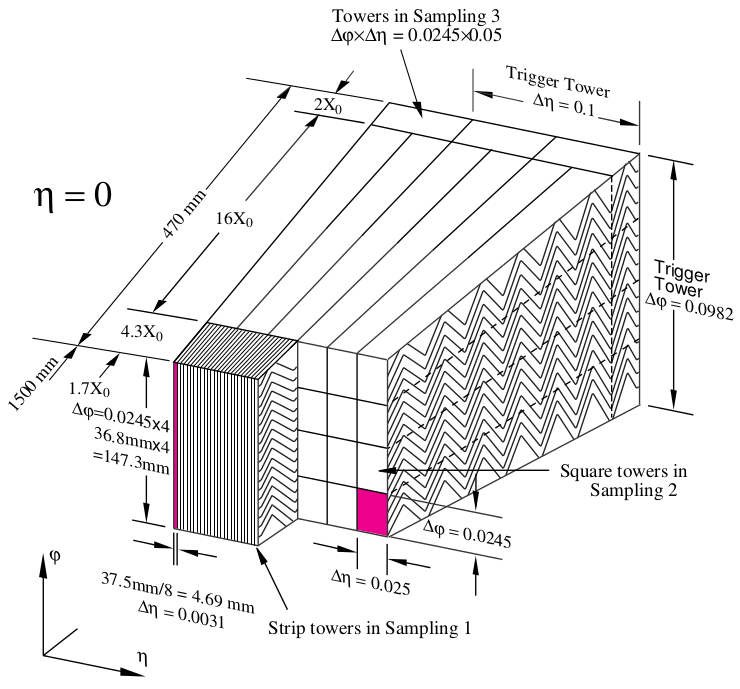
\includegraphics[width=0.7\textwidth]{img/accordion}
    \caption[Schematischer Ausschnitt des elektromagnetischen Kalorimeters]
        {Schematische Ausschnitt des elektromagnetischen Kalorimeters im
        Bereich des Barrel. Zu sehen sind alle drei Lagen und die angedeutete
        Akkorden-Geometrie.}
    \label{fig:accordion}
\end{figure}

Das Barrel ist aus drei Lagen unterschiedlicher Dicke aufgebaut, die in Abb.
\ref{fig:accordion} mit \textit{Sampling 1,2,3} bezeichnet werden. Die erste
dieser Lagen hat eine besonders feine Unterteilung $\eta$ von $0,0031$, was zum
einen zu einer guten Positionsauflösung in dieser Richtung führt und zum
anderen zur Unterscheidung nahe beieinander eintreffender Teilchen genutzt
wird\footnote{beispielweise zwei Photonen aus dem eines Pions kurz vor dem
Kalorimeter}. Die Stärke dieser Schicht beträgt etwa $4,3$ Strahlungslängen
($X_0$). Die zweite Lage hingegen ist gröber in $\eta$, jedoch feiner in $\phi$
granuliert und stellt mit 16 Strahlungslängen ($X_0$) die größte der Lagen dar.
Mit ihr soll der Großteil der Energiedeposition erfasst werden. Den äußeren
Rand bildet die dritte und letzte Lage, die nochmals gröber in unterteilt und
mit gerademal 2 Strahlungslängen Dicke die kürzeste der drei Lagen ist. Deren
Aufgabe ist es, über das elektromagnetische Kalorimeter hinaus ins hadronische
Kalorimeter übersprechende Energiedepositionen abzuschätzen. Vor den hier
beschriebenen drei Lagen\footnote{\textit{vor} meint hier aus Sicht der
Strahlachse} befindet sich noch eine einzige Schicht aus flüssigen Argons, die
den sogenannten \textit{Presampler} bildet und zur Korrektur der vor dem
Kalorimeter deponierten Energie dient.

Links und rechts des Barrels schließen sich die Endkappen-Kalorimeter an (siehe
Abb. \ref{fig:calorimeter}), die kurz mit EMEC\footnote{\acf{EMEC}} bezeichnet
werden. Diese Wagenrad förmigen Kontrukte bestehen jeweils aus einem inneren
und einem äußeren Teil, wobei der äußere Teil einen Bereich von
$1.375<|\eta|<2.5$ abdeckt und damit nach der Definition vom Beginn dieses
Abschnitts gerade noch zum Zentral-Bereich gehört. Dementsprechend zählt der
innere Teil ($2.5<|\eta|<3.2$) bereits zum Vorwärts-Bereich. Wie schon im
Barrel werden im gesamten \ac{EMEC} die Bleiabsorber-Schichten in
Akkorden-Struktur verwendet, welche hier jedoch orthogonal zur Strahlachse
ausgerichtet sind. Der äußere Bereich besteht dabei analog zum Barrel aus drei
Lagen mit vergleichbarer Granularität. Der innere Bereich hingegen besteht nur
aus den hinteren beiden Lagen  und ist mit $0,1\times0,1$ in $\eta\times\phi$
deutlich gröber segmentiert.

Der letzte Teil des elektromagnetischen Kalorimeters befindet sich weit im
Vorwärts-Bereich zwischen $3.0<|\eta|<4.9$ und wird deshalb \acf{FCal} genannt.
Als Absorber-Material wurde hier eine Matrix aus Kupfer gewählt, in die
hexagonal angeordnete Röhren förmige Öffnungen eingelassen sind (siehe
Abbildung \ref{fig:fcal}).
\begin{figure}[h]
    \centering
    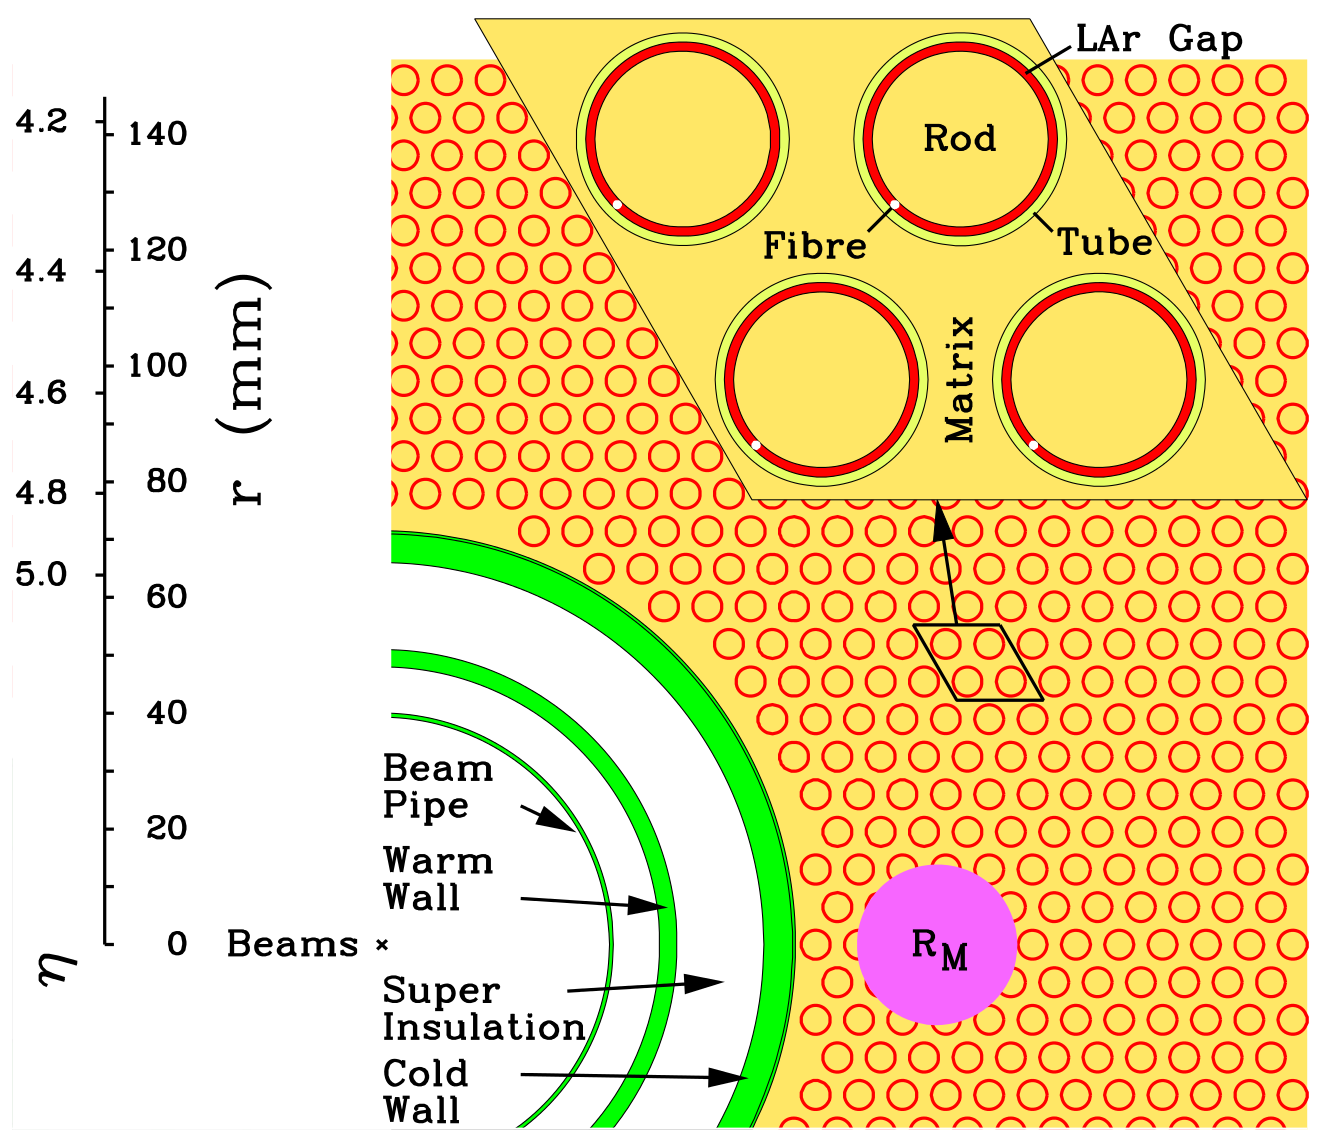
\includegraphics[width=0.6\textwidth]{img/fcal}
    \caption[]{}
    \label{fig:fcal}
\end{figure}
In die Röhren wiederum wurden Kupferstäbe mit einem etwas kleineren Durchmesser
eingebracht, die von Quarzfasern spiralförmig umgeben im Zentrum der Röhren
gehalten werden. Die Lücke zwischen den Stäben und der Matrix von
$0,25\milli\meter$ Größe wird durch flüssiges Argon als Nachweismedium
gefüllt. Die Kupferstäbe stehen gegenüber der Matrix unter positiver
Hochspannung und fungieren somit als Elektroden. Die Skala auf der linken Seite
von Abb. \ref{fig:fcal} deutet im Vergleich mit den auf der rechten Seite
dargestellten Röhren bereits an, dass die Granularität hier deutlich gröber
ist, als für die übrigen Teile des Kalorimeters. Die hier vorherrschende
deutliche höhere Strahlenbelastung macht dies aber notwendig.

\subsubsection{Das hadronische Kalorimeter}
Das hadronische Kalorimeter umschließt sein elektromagnetisches Pendant und
arbeitet nach einem ähnlichen Prinzip. Allerdings werden hier im
Zentral-Bereich Eisenkacheln als Absorber und ein Szintillator als aktives
Nachweismedium benutzt.



\subsection{Trigger und DAQ}
\label{trigger_daq}
Beim Betrieb des \ac{LHC} mit Design-Parametern findet alle $25\nano\second$
die Kollision zweier Proton-Pakete statt. Eine solche Kollision führt im Mittel
zu über 20 gleichzeitigen Interaktionen, was in einer Gesamt-Interaktionsrate
von rund $1\giga\hertz$ resultiert. Die Aufgabe des ATLAS Trigger-Systems ist
es diese Flut an Ereignissen auf ein Maß zu reduzieren, auf dem es möglich ist,
die gewonnenen Daten zu Verarbeiten und zu Speichern, was bei etwa $200\hertz$
der Fall ist. Das Trigger-System soll dabei möglichst die interessanten und
seltenen Ereignisse selektieren, während es uninteressante Ereignisse verwirft.

Die Reduktion der Rate um sieben Größenordnungen geschieht in drei Stufen.
Als erstes erfolgt eine hardware-basierte Prüfung, die schlicht Level-1 genannt
wird und die Rate bereits auf $75\kilo\hertz$ reduziert. Dem Level-1 Trigger
stehen dazu nur die groben Informationen aus den, Kalorimetern und Myon-Kammern
zur Verfügung. Es werden dabei sogenannte \acf{ROI}, also Regionen von
besonderem Interesse, gebildet und nach deren Multiplizität bzw. einfachen
kinematischen Eigenschaften entschieden\footnote{z.B. 2 Elektronkandidaten mit
einem transveralen Impuls größer $20\GeV$}. Ihm bleiben dafür nicht mehr als
$2,5\micro\second$ Zeit. Fällt die Entscheidung positiv aus, übernimmt die
nächste Stufe, der software gestützte Level-2 Trigger, die weitere Prüfung der
\ac{ROI} in voller Granularität und unter Einbeziehung der Spurinformationen.
Nach etwa $40\micro\second$ muss eine Entscheidung gefällt sein, wodurch die
Ereignisrate auf etwa $2\kilo\hertz$ reduziert wird. Die dritte und letzte
Stufe ist der sogenannte \acf{EF}, der ebenfalls software-basiert komplexere
Rekonstruktionsalgorithmen anwendet und auch außerhalb der \ac{ROI} die volle
Detektorinformation zur Verfügung hat. Die Zeit für eine Entscheidung liegt bei
einigen Sekunden, und die Rate wird auf die angestrebten $200\hertz$ reduziert.

Fällt auch die letzte Triggerentscheidung positiv aus werden alle Informationen
des Ereignisses als Roh-Daten abgespeichert.


\pagebreak


%______________________________________________________________________________
%                                                           Elektronen in ALTAS
%
\section{Elektronen in ATLAS}
\label{electrons}

In diesem Abschnitt wird erläutert, wie Elektronen und Positronen in ATLAS
identifziert und rekonstruiert werden. Dabei kann ein Einblick in die
prinzipielle Funktionsweise des Detektors im Sinne des Nachweises von Teilchen
gewonnen werden. Es wird zunächst kurz der Weg eines Elektrons oder Positrons
von Entstehung im Streuprozess bis zu dessen Absorption im Kalorimeter
beschrieben, bevor auf die Einzelheiten der Rekonstrukton näher eingegangen
wird.

In dieser Arbeit wird der Drell-Yan Prozess\footnote{siehe Kapitel
\ref{theory:afb}} betrachtet, bei dem ein Z-Boson erzeugt wird, welches
anschließend in ein Paar aus Elektron und Positron zerfällt. Aufgrund der
kurzen Lebensdauer des Z-Bosons findet dieser Zerfall sehr nahe am
ursprünglichen Kollisionspunkt des Quark-Antiquark Paares statt. Abhängig vom
Lo"-rentz-Boost des Z-Bosons treten Elektron und Positron nun in
unterschiedlichen Richtungen in das Spursystem ein, wo sie entsprechend ihrer
Ladung aufgrund des solenoiden Magnetfeldes auf eine gekrümmte Flugbahn
gezwungen werden\footnote{einzige Ausnahme stellen Elektronen bzw. Positronen
dar, die in Vorwärts-Richtung ($|\eta|>2.5$) emittiert wurden. In diesem
Bereich exisitiert kein Spursystem (siehe Abschnitt \ref{inner_detector})},
welche durch das Spursystem nachgewiesen wird. Aus der Krümmung der Spur und
der Richtung des Magnetfeldes lässt sich die Ladung und der Impuls des
Elektrons bzw. Positrons bestimmen. Ab diesem Punkt verhalten sich Elektronen
und Positronen gleich, weshalb im Folgenden nicht mehr zwischen ihnen
unterschieden wird und schlichtweg von Elektronen gesprochen wird. Nach dem
Spursystem treten die Elektronen in das elektromagnetische Kalorimeter ein, wo
sie unter ständigem Verlust von Energie einen Teilchenschauer induzieren (siehe
Abschnitt \ref{calorimeter}). Dieser wird im Folgenden als \textit{Cluster}
bezeichent. Idealerweise werden die Elektronen im Kalorimeter vollständig
gestoppt, sodass keine Energie in das dahinterliegende hadronische Kalorimeter
entweicht.



\subsection{Rekonstruktionsalgorithmen}
\label{reconstruction}
Die Rekonstruktion der Elektronen im Zentral-Bereich beginnt mit der Suche nach
zusammenpassenden Spuren und Clustern. Dabei kann von beiden Seiten begonnen
werden, d.h. entweder man sucht zu einem Cluster die passende Spur oder zu
einer Spur den passenden Cluster. Beide Fälle sind als
Rekonstruktionsalgorithmen implementiert und werden kurz \textit{eGamma}- bzw.
\textit{softe}-Algorithmus genannt. Eine Spur gilt vorerst als dann zu einem
Cluster passend, wenn die Distanz in der $\eta\times\phi$-Ebene zwischen Spur
und Cluster in einem Wert von $0,05\times0,10$ nicht überschreitet.

Zum primären Auffinden von Clustern im Kalorimeter verwendet der
eGamma-Algorithmus ein verschiebbares virtuelles Fenster von $3\times5$ Zellen
Größe. Übersteigt die Summe der Energie innerhalb dieses Fensters einen Wert
von $2,5\GeV$, wird der Cluster als Elektronkandidat angesehen und die Suche
nach einer passenden Spur begonnen. Werden dabei mehr als eine passende Spur
identifiziert, so wird jene mit dem geringsten Abstand in $\eta\times\phi$
gewählt. Wird im Gegenteil keine Spur gefunden, die auf den Cluster zeigt, wird
dieser als Elektronkandidat verworfen. Allgemein eignet sich der
eGamma-Algorithmus für einen großen Bereich der Energie. Der softe-Algorithmus
hingegen beginnt umgekehrt mit der Suche eines Clusters zu einer bereits
rekonstruierten Spur, weshalb er besonders für niederenergetische Elektronen
geeignet ist. Alle erfolgreichen Spur-Cluster Zuordnungen werden anschließend
als Elektronkandidaten weiter betrachtet.

Im Vorwärts-Bereich, der über kein Spursystem verfügt, erfolgt die Auffindung
von Elektronkandidaten rein über die Cluster-Information im Kalorimeter. Aus
diesem Grund kann hier primär nicht zwischen Photonen und Elektronen
unterschieden werden.



\subsection{Elektronidentifikation}
\label{identification}
Die durch die Rekonstruktionsalgorithmen deklarierten Elektronkandidaten
sind allerdings noch durch einen Großteil sich ähnlich verhaltender Teilchen,
wie Pionen oder leichte Jets kontaminiert. Deshalb führt man weitere Kriterien
ein, um zwischen echten Elektronen und Untergrundteilchen zur unterscheiden.
Die Kriterien werden dabei in drei hierarchisch abgestuften Kategorien
definiert, wobei eine höhere Kategorie stets alle Kriterien einer niedrigeren
Kategorie enthält. Umso höher die Kategorie desto größer die Unterdrückung
andersartiger Teilchen. Im Gegenzug wächst allerdings auch die
Wahrscheinlichkeit echte Elektronen zu verwerfen. Bei der Definition der
Identifikations-Kategorien (kurz: \acs{ID}) muss erneut zwischen Zentral-
($|\eta|<2.5$) und Vorwärts-Elektronen ($2.5<|\eta|<4.9$) unterschieden werden.

Die drei Kategorien für Zentral-Elektronen heißen \textit{loose++},
\textit{medium++} und \textit{tight++}. Die loose++ ID beinhalten Schnitte auf
die Schauerform in der ersten und zweiten Lage des Kalorimeters\footnote{siehe
Abschnitt \ref{calorimeter}}, sowie den longitudinalen Verlust von Energie in
die erste Lage des hadronischen Kalorimeters. Desweiteren wird mindestens ein
Spurtreffer im Pixeldetektor und sechs weitere im Silizium-Streifen Detektor
gefordert. Die medium++ ID implementiert, wie bereits erwähnt alle Schnitte von
loose++, jedoch mit stärken Schnittgrenzen. Zudem werden als weitere Kriterien
ein Treffer in der ersten Lage des Pixel-Detektors (b-Layer) und eine genauere
Übereinstimmung zwischen Spur und Cluster-Position eingeführt. Für die höchste
Stufe, tight++, werden die vorangegangen Schnittwerte nochmal angehoben und nun
auch Spurtreffer im \ac{TRT} gefordert. Außerdem ist nun auch ein bestimmtes
Verhältnis zwischen Cluster-Energie und Impuls ($E/p$) notwendig.

Für Vorwärts-Elektronen wählt man analoge Bezeichner für die ID-Kategorien:
\linebreak
\textit{fwdLoose}, \textit{fwdMedium} und \textit{fwdTight}. Die Kriterien
dieser Kategorien basieren aufgrund der fehlenden Spurinformation und der
besonderen Geometrie der Vorwärs-Kalorimeter rein auf der Form und der
Energieverteilung der Cluster. Zu den insgesammt sechs Observablen auf denen
die Schnittkriterien defniert sind zählt der Abstand des Cluster-Schwerpunkts
von der der Stirnseite des Kalorimeters, der Anteil der Energie in der
hochenergetischsten Zelle gemessen am Cluster als ganzes, das laterale und
longitudinale Cluster-Moment zweiter Ordnung, sowie deren normalisiertes
Pendant. Die Cluster-Momente sind dabei definiert als
\begin{equation}
    \langle x^n \rangle = \frac{\sum_i E_i x_i^n}{\sum_i E_i}
\end{equation}
wobei x die entweder die longitudinale oder laterale Enterfernung der i-ten
Zelle eines Clusters zu dessen Zentrum ist und $E_i$ die in dieser Zelle
deponierte Energie. $n$ bestimmt die Ordnung des Moments. Da die Schnitte auf
diese sechs Größen aus der multi-variaten Berechnung einer
Fischer-Diskriminanten hervorgehen, macht es hier keinen Sinn feste Grenzen
anzugeben.

